\documentclass[border=5mm]{standalone}
\usepackage{pgfplots}
\pgfplotsset{compat=1.18}
\usepackage{xcolor}

\begin{document}
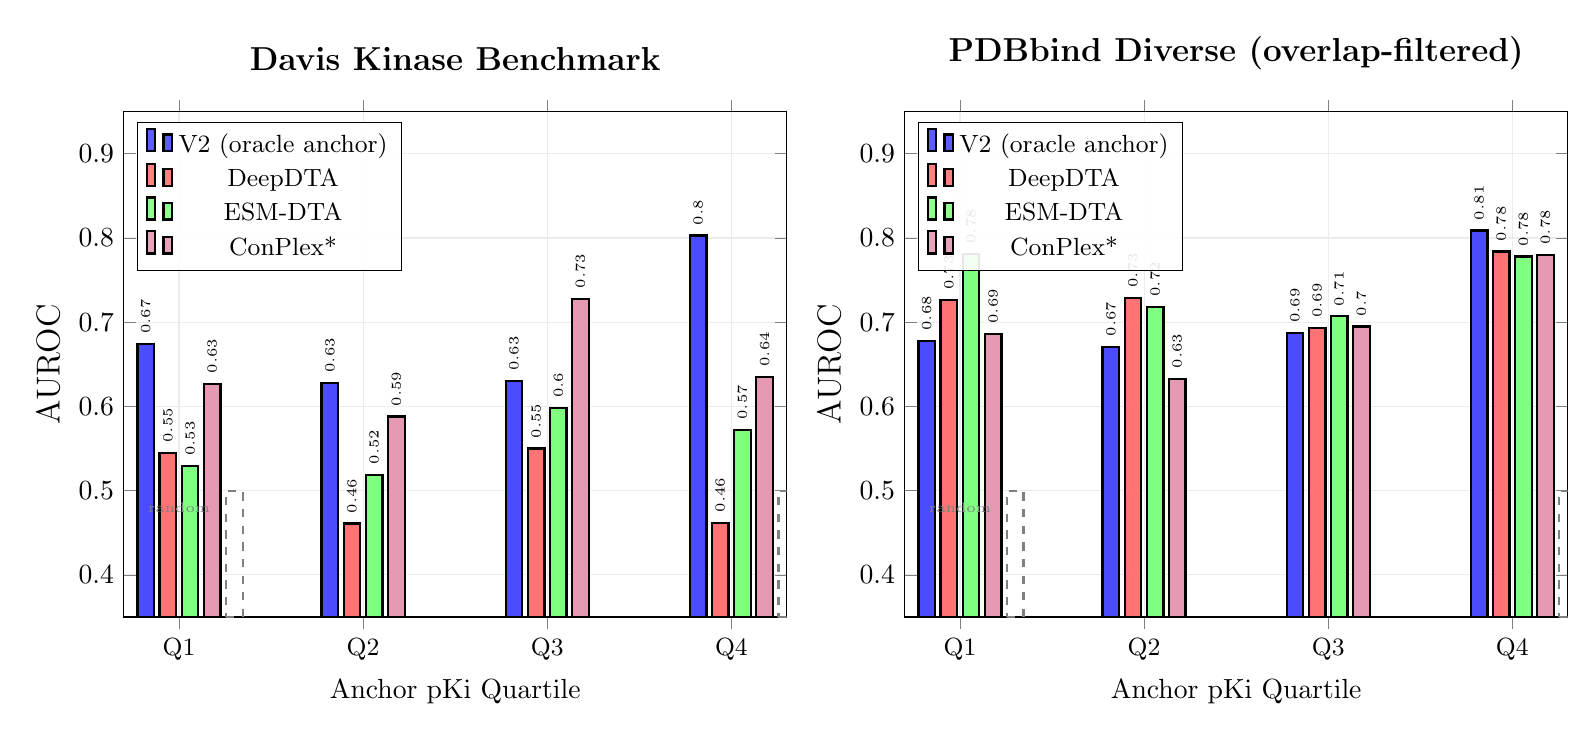
\begin{tikzpicture}

% ── DAVIS (left panel) ──
\begin{axis}[
    name=davis,
    ybar,
    bar width=6pt,
    width=10cm,
    height=8cm,
    ylabel={AUROC},
    ylabel style={font=\large},
    xlabel={Anchor pKi Quartile},
    xlabel style={font=\normalsize},
    symbolic x coords={Q1, Q2, Q3, Q4},
    xtick=data,
    x tick label style={font=\small},
    ymin=0.35, ymax=0.95,
    legend style={at={(0.02,0.98)}, anchor=north west, font=\small, legend columns=1, fill=white, fill opacity=0.9, draw opacity=1, text opacity=1},
    title={\textbf{Davis Kinase Benchmark}},
    title style={font=\large, at={(0.5,1.03)}, anchor=south},
    grid=major,
    grid style={gray!15},
    ymajorgrids=true,
    every axis plot/.append style={thick},
    nodes near coords style={font=\tiny, rotate=90, anchor=west},
]

% V2 Oracle
\addplot[fill=blue!70, nodes near coords] coordinates {
    (Q1, 0.674) (Q2, 0.628) (Q3, 0.630) (Q4, 0.803)
};

% DeepDTA
\addplot[fill=red!55, nodes near coords] coordinates {
    (Q1, 0.545) (Q2, 0.461) (Q3, 0.550) (Q4, 0.462)
};

% ESM-DTA
\addplot[fill=green!50, nodes near coords] coordinates {
    (Q1, 0.529) (Q2, 0.519) (Q3, 0.598) (Q4, 0.572)
};

% ConPlex
\addplot[fill=purple!40, nodes near coords] coordinates {
    (Q1, 0.627) (Q2, 0.588) (Q3, 0.728) (Q4, 0.635)
};

\legend{V2 (oracle anchor), DeepDTA, ESM-DTA, ConPlex*}

% Random baseline
\addplot[dashed, gray, thick, forget plot] coordinates {(Q1, 0.5) (Q4, 0.5)};
\node[font=\tiny, gray] at (axis cs:Q1, 0.48) {random};

% Quartile ranges as x-axis subtitle
\node[font=\tiny, gray, anchor=north] at (axis cs:Q1, 0.35) {pKi 5--8};
\node[font=\tiny, gray, anchor=north] at (axis cs:Q2, 0.35) {pKi 8--9};
\node[font=\tiny, gray, anchor=north] at (axis cs:Q3, 0.35) {pKi 9--9.2};
\node[font=\tiny, gray, anchor=north] at (axis cs:Q4, 0.35) {pKi 9.2--11};

\end{axis}

% ── PDBbind (right panel) ──
\begin{axis}[
    at={(davis.east)},
    anchor=west,
    xshift=1.5cm,
    ybar,
    bar width=6pt,
    width=10cm,
    height=8cm,
    ylabel={AUROC},
    ylabel style={font=\large},
    xlabel={Anchor pKi Quartile},
    xlabel style={font=\normalsize},
    symbolic x coords={Q1, Q2, Q3, Q4},
    xtick=data,
    x tick label style={font=\small},
    ymin=0.35, ymax=0.95,
    legend style={at={(0.02,0.98)}, anchor=north west, font=\small, legend columns=1, fill=white, fill opacity=0.9, draw opacity=1, text opacity=1},
    title={\textbf{PDBbind Diverse (overlap-filtered)}},
    title style={font=\large, at={(0.5,1.03)}, anchor=south},
    grid=major,
    grid style={gray!15},
    ymajorgrids=true,
    every axis plot/.append style={thick},
    nodes near coords style={font=\tiny, rotate=90, anchor=west},
]

% V2 Oracle (from overlap-filtered run, n=5731)
\addplot[fill=blue!70, nodes near coords] coordinates {
    (Q1, 0.678) (Q2, 0.671) (Q3, 0.687) (Q4, 0.809)
};

% DeepDTA
\addplot[fill=red!55, nodes near coords] coordinates {
    (Q1, 0.726) (Q2, 0.729) (Q3, 0.693) (Q4, 0.784)
};

% ESM-DTA
\addplot[fill=green!50, nodes near coords] coordinates {
    (Q1, 0.781) (Q2, 0.718) (Q3, 0.707) (Q4, 0.778)
};

% ConPlex
\addplot[fill=purple!40, nodes near coords] coordinates {
    (Q1, 0.686) (Q2, 0.633) (Q3, 0.695) (Q4, 0.780)
};

\legend{V2 (oracle anchor), DeepDTA, ESM-DTA, ConPlex*}

% Random baseline
\addplot[dashed, gray, thick, forget plot] coordinates {(Q1, 0.5) (Q4, 0.5)};
\node[font=\tiny, gray] at (axis cs:Q1, 0.48) {random};

% Quartile ranges
\node[font=\tiny, gray, anchor=north] at (axis cs:Q1, 0.35) {pKi 1--6};
\node[font=\tiny, gray, anchor=north] at (axis cs:Q2, 0.35) {pKi 6--7};
\node[font=\tiny, gray, anchor=north] at (axis cs:Q3, 0.35) {pKi 7--9};
\node[font=\tiny, gray, anchor=north] at (axis cs:Q4, 0.35) {pKi 9--15};

\end{axis}

\end{tikzpicture}
\end{document}
